\documentclass[Master]{subfiles}
\begin{document}
\section{2D Chiral Topological P-Wave Superconductor}\label{sec:2DTopSuper}
Given spin less fermions on a 2D lattice with hopping term $t$, Chemical Potential $\mu$ and a superconducting oder parameter $\Delta$ with orthogonal phase in x and y direction.
The Hamiltonian of this model, sometimes also called 2D $(p_x + i p_y)$ superconductor takes the form.
\begin{dmath}\label{math:Hamil_MultiPart}
\hat{H} = \sum_{m,n} \left[-t\left((c_{m+1,n}^{\dag}c_{m,n}+h.c.)
+ (c_{m,n+1}^{\dag}c_{m,n}+h.c.)
\right)
-\mu c_{m,n}^{\dag} c_{m,n} 
+ ( \Delta c_{m+1,n}^{\dag}c_{m,n}^{\dag} + \Delta^* c_{m,n}c_{m+1,n})
+ i( \Delta c_{m,n+1}^{\dag}c_{m,n}^{\dag} -\Delta^* c_{m,n}c_{m,n+1})
\right]
\end{dmath}

Similar to the 1D Kitaev chain \cite{kitaev2001unpaired} this model is a superconductor with a topological phase. 
The lattice Hamiltonian can be Fourier transformed and written in Bogoliubov de Gennes form:

\begin{dmath}\label{math:HamilBdG}
\hat{H}_{BdG} = 
\frac{1}{2}
\sum_{\vec{p}} 
\Psi_{\vec{p}}^{\dag}
\left(
\begin{array}{cc}
\epsilon(\vec{p}) & 2 i \Delta( \sin \ p_x + i \sin \ p_y)\\
-2 i \Delta^*( \sin \ p_x - i \sin \ p_y) & - \epsilon(\vec{p})
\end{array}
\right)
\Psi_{\vec{p}}
\end{dmath}
with $\epsilon(\vec{p}) = -2t ( \cos p_x + \cos p_y) - \mu $ and $\Psi = (\hat{c}_{\vec{p}},\hat{c}_{\vec{-p}}^{\dag})^T$.\\
With a $U(2)$ gauge transformation on the $c_{vec{p}}$ operators, the complex phase of $\Delta$ can be absorbed.
$$
\Delta = |\Delta| e^{i \theta} : c_{vec{p}} \rightarrow  e^{i \theta /2} c_{vec{p}}
$$
Then the Hamiltonian can be decomposed in the Pauli-matrix basis as:
$$
\hat{H}_{BdG} =  \epsilon(\vec{p}) \sigma^z - 2 |\Delta|\sin \ p_x \sigma^y -2 |\Delta|\sin \ p_y \sigma^x = \vec{d} \cdot \boldsymbol\sigma
$$
Thus, the $\vec{d}$ vector is 
$$
\vec{d}=\left(
\begin{array}{c}
     - 2 |\Delta|\sin \ p_y\\
     -2 |\Delta|\sin \ p_x\\
   -2t (cos \ p_x +\cos\  p_y) - \mu
\end{array}\right)
$$
The quasi-partice spectrum of this model is 
$$
E_{\pm}(\vec{p}) = \pm \sqrt{(-\mu - 2 t (cos \ p_x +\cos \ p_y))^2+ 4|\Delta|^2 (sin^2 \ p_x +\sin^2 \ p_y)}
$$
When $ \Delta = 0$, the spectrum simplifies to $ E = \pm (-\mu - 2 t (cos \ p_x +cos \ p_y))$, for which there is always a root for $|\frac{\mu}{t}| \leq 4 $ as $ |cos \ p_x -cos \ p_y| < 2$ Otherwise the spectrum is gapped.\\
Even when $\Delta \neq 0$ the gap in the spectrum closes at three different points $\frac{\mu}{t} = \{-4,0,4\}$. These points mark the topological phase transitions:

\begin{figure}[H]
\minipage[t]{0.3\textwidth}
  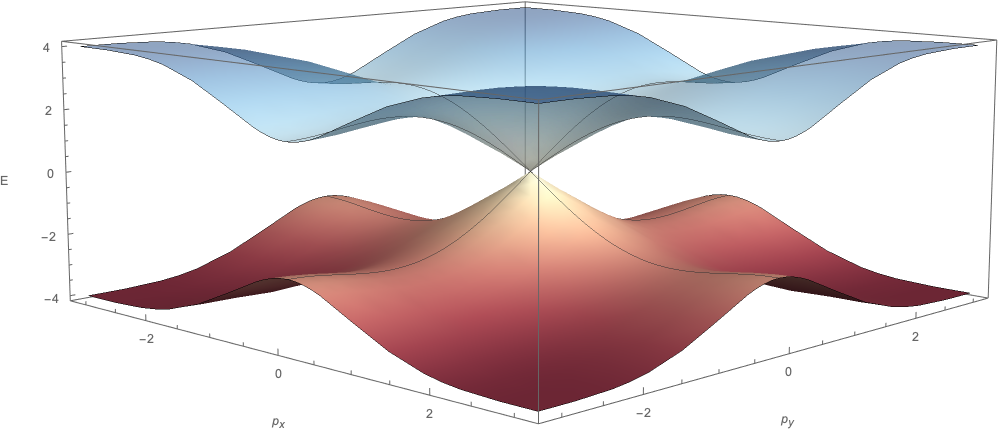
\includegraphics[scale=0.15]{imgs/SpektrumDelta1Mu0.png}
  \centering
  $\mu = -2$\\
\endminipage\hfill
\minipage[t]{0.3\textwidth}
  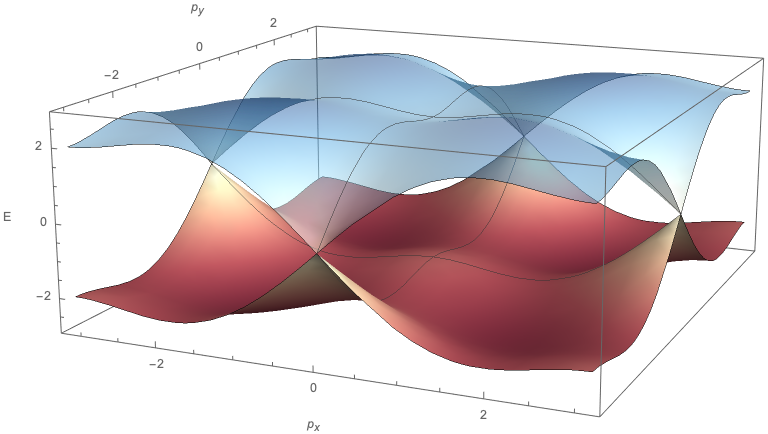
\includegraphics[scale=0.17]{imgs/SpektrumDelta1Mu2.png}
  \centering
  $\mu = 0$\\
\endminipage\hfill
\minipage[t]{0.3\textwidth}%
  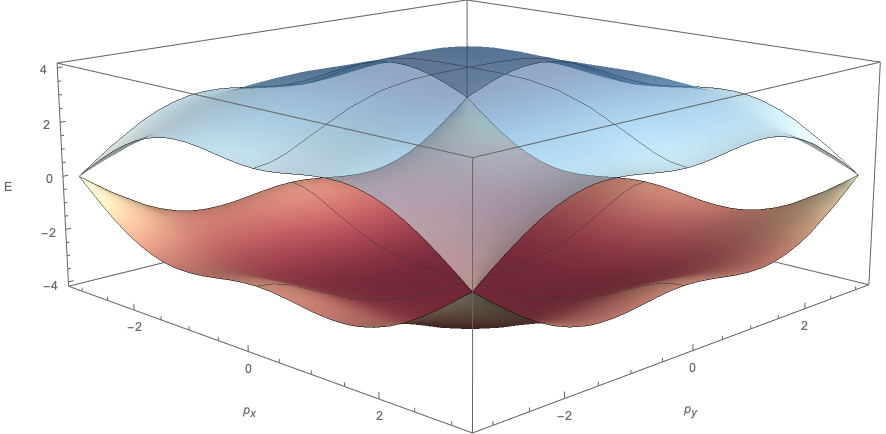
\includegraphics[scale=0.16]{imgs/SpektrumDelta1Mu4.png}
  \centering
  $\mu = 2$\\
\endminipage
\caption{Plots of the Spectrum roots for $\Delta = 1 , t = 1/2$}
\end{figure}
\subsection{Symmetries}
The BdG Hamiltonian has no time reversal symmetry $\mathcal{T}$ but an induced charge conjugation symmetry (see \secref{sec:indChegeConjSym}) of the from $\mathcal{C} = \sigma^x K$, where $K$ is the complex conjugation operator.
$$
\mathcal{C}H_{BdG} = \sigma^x K \vec{d} \cdot \boldsymbol\sigma = \sigma^x \vec{d}^* \cdot \boldsymbol\sigma^* = - \vec{d} \cdot \boldsymbol\sigma \sigma^x  = - H_{BdG} \mathcal{C}
$$
The $\mathcal{C}^2$ symmetry squares to one: 
$$\mathcal{C}^2 = \sigma^x(\sigma^x)^* = +\mathbb{1}_2$$
A chiral symmetry $\mathcal{S} = \mathcal{T}\mathcal{C}$ cannot exit when only one of the $\mathcal{T},\mathcal{C}$ symmetries exists.
Thus, the Hamiltonian is of type $\mathbf{D}$ in the Cartan Classification. Therefore, a $\mathbb{Z}$ topological invariant classifies the Hamiltonian\cite{PhysRevB.55.1142} calculated by the  winding number.

\subsection{Topological Phases}\label{sec:HamilPhases}
This Hamiltonian has four topologial regimes. The two regimes where $|\frac{\mu}{t}|>4$, are topologically trivial whereas the two regimes $0<\frac{\mu}{t}<4$ and $-4<\frac{\mu}{t}<0$ are topological and have opposed chirality.
As the gap is open for $|\frac{\mu}{t}|<4$ for both $\Delta = 0$ and $\Delta \neq 0$ these phases are connected and, thus, topologically the same. Whereas the gapped $0<\frac{\mu}{|t|}<4$ and $0>\frac{\mu}{|t|}>-4$ phases cannot be connected to any other phase without passing a critical (non gapped) region. Therefore, they are, topologically distinct.


\begin{figure}[H]
\centering 
\minipage[t]{0.48\textwidth}
\centering
\hspace{.45cm}$\Delta = 0$
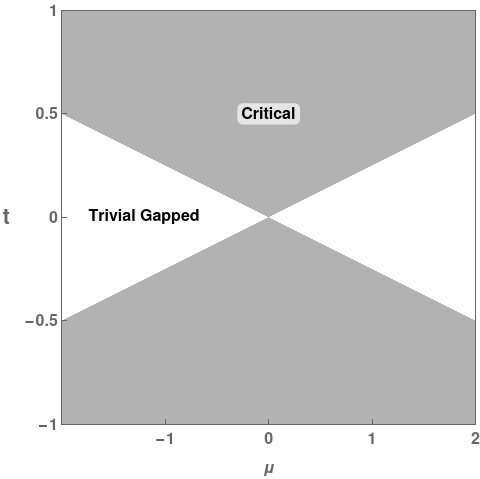
\includegraphics[width=\linewidth]{imgs/Phase_Diagramm_Trivial.png}
\endminipage\hfill
\minipage[t]{0.48\textwidth}
\centering
\hspace{.35cm}$\Delta \neq 0$
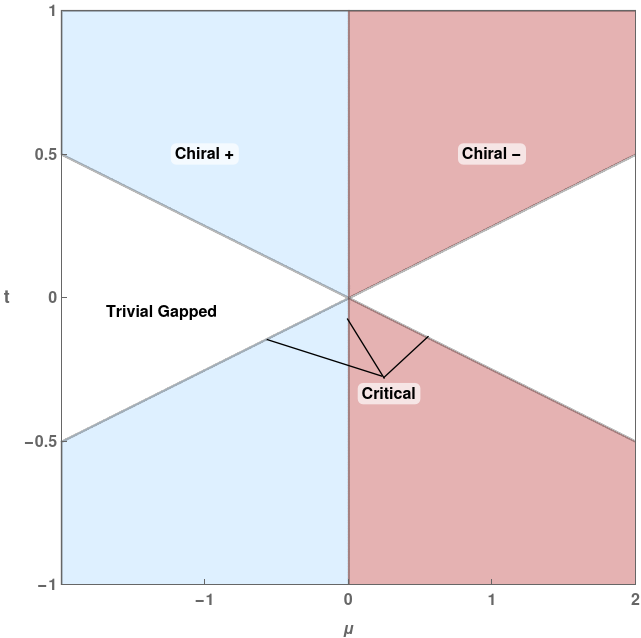
\includegraphics[width=\linewidth]{imgs/Phase_Diagramm.png}
\endminipage
\caption{Phase diagram of the Hamiltonian \eqref{math:HamilBdG} in the topological and non-topological regimes depending on $\mu$ and $t$}
\label{fig:Phase_Diagramm}
\end{figure}


Each of the three critical strips can be mapped to the $ \mu = 0 $ line by a mapping $\mu \rightarrow \mu \pm 4t$. Then the critical points are at $\frac{\mu}{t} = \{-4,0,4\} \pm 4$.


\begin{figure}[H]
\centering
\minipage[t]{0.4\textwidth}
\centering
\hspace{.35cm}$\mu \rightarrow \mu + 4t$\\
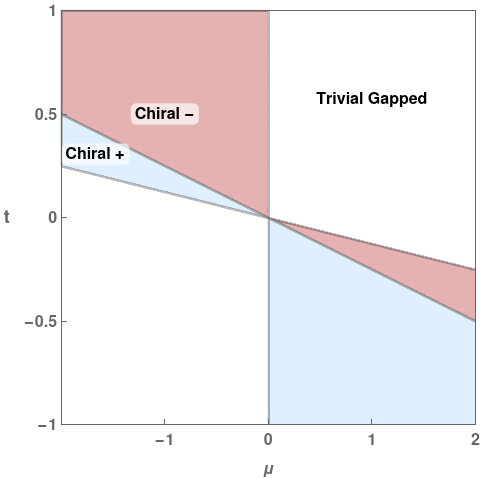
\includegraphics[width=\linewidth]{imgs/Phase_Diagramm+4t.png}
\endminipage\hspace{1cm}
\minipage[t]{0.4\textwidth}
\centering
\hspace{.35cm}$\mu \rightarrow \mu - 4t$\\
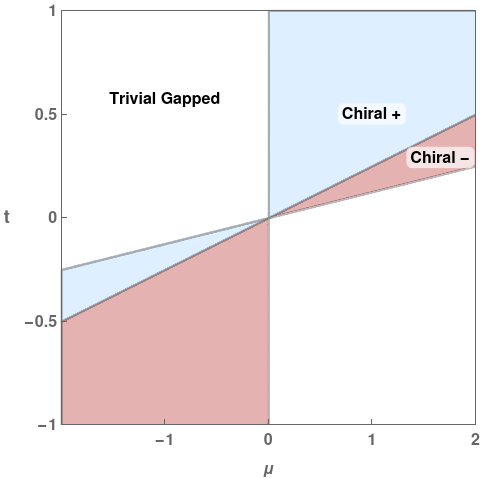
\includegraphics[width=\linewidth]{imgs/Phase_Diagramm-4t.png}
\endminipage
\caption{Phase diagram of the Hamiltonian \eqref{math:HamilBdG} in the topological $\Delta \neq 0$ regimes depending on $\mu$ and $t$}
\label{fig:Phase_Diagramm+-4t}
\end{figure}
The topological invariant for a 2D \textbf{D} type Hamiltonian is given by the winding number and computes as:
$$
\mathcal{N} = \frac{1}{8\pi} \int d\vec{p} \ \frac{\ \epsilon_{i j} \ \vec{d}\cdot (\partial p_i \vec{d}\cross \partial p_j \vec{d})}{|d|^3} 
$$
$$= \frac{1}{8\pi} \int_{-\pi}^{\pi} dp_x \int_{-\pi}^{\pi} dp_y \frac
{8 |\Delta| ^2 \left(\mu \cos \ p_x  \cos \ p_y + 2 t (\cos \ p_x + \cos \ p_y)\right)}
{\left(4 |\Delta| ^2 (\sin ^2\ p_x+ \sin ^2\ p_y)+(\mu +2 t (\cos \ p_x+ \cos \ p_y))^2\right)^{3/2}}
$$
This integral can be evaluated numerically as in  \figref{fig:WindingNumbe_Diagramm} to confirm the phase diagram \figref{fig:Phase_Diagramm}.
\begin{figure}[H]\label{fig:WindingNumber_Diagramm}
\centering
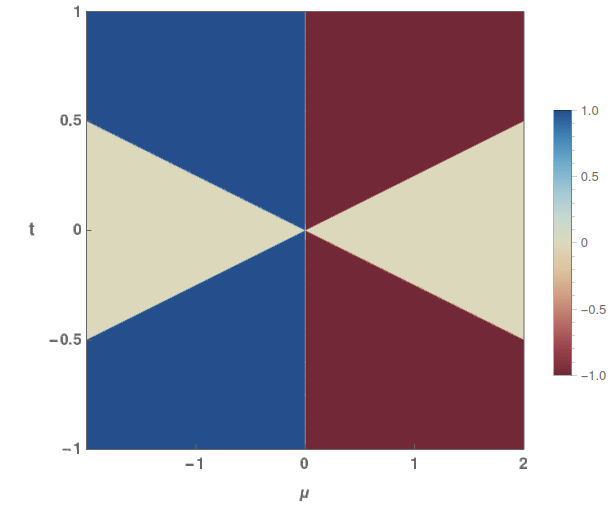
\includegraphics[width=.6\linewidth]{imgs/Winding_Diagramm.png}
\caption{Numerical evaluation of  Winding number of the Hamiltonian \eqref{math:HamilBdG} for $|\Delta| = 1$ depending on $\mu$ and $t$}
\label{fig:WindingNumbe_Diagramm}
\end{figure}
\subsection{Vortex Bound States}\label{sec:VBS}
When two spatially extended but topologically distinct regions are joined by an interface as is the case in \secref{sec:BulkEdgeCorrespondance}, zero-energy modes occur. For the 2D Chiral Topological P-Wave Superconductor \secref{sec:2DTopSuper} the edge-modes on 1D line interfaces are predicted to be a chiral Majorana modes (see \figref{fig:TopLineDefects}). Thus, they have momentum along the interface. Additional fermionic modes appear in the superconductor gap equally-spaced around zero energy \cite{volovik1999fermion}: 
\begin{figure}[H]
\centering
\minipage[t]{0.4\textwidth}
\centering
\fcolorbox{black}{white}{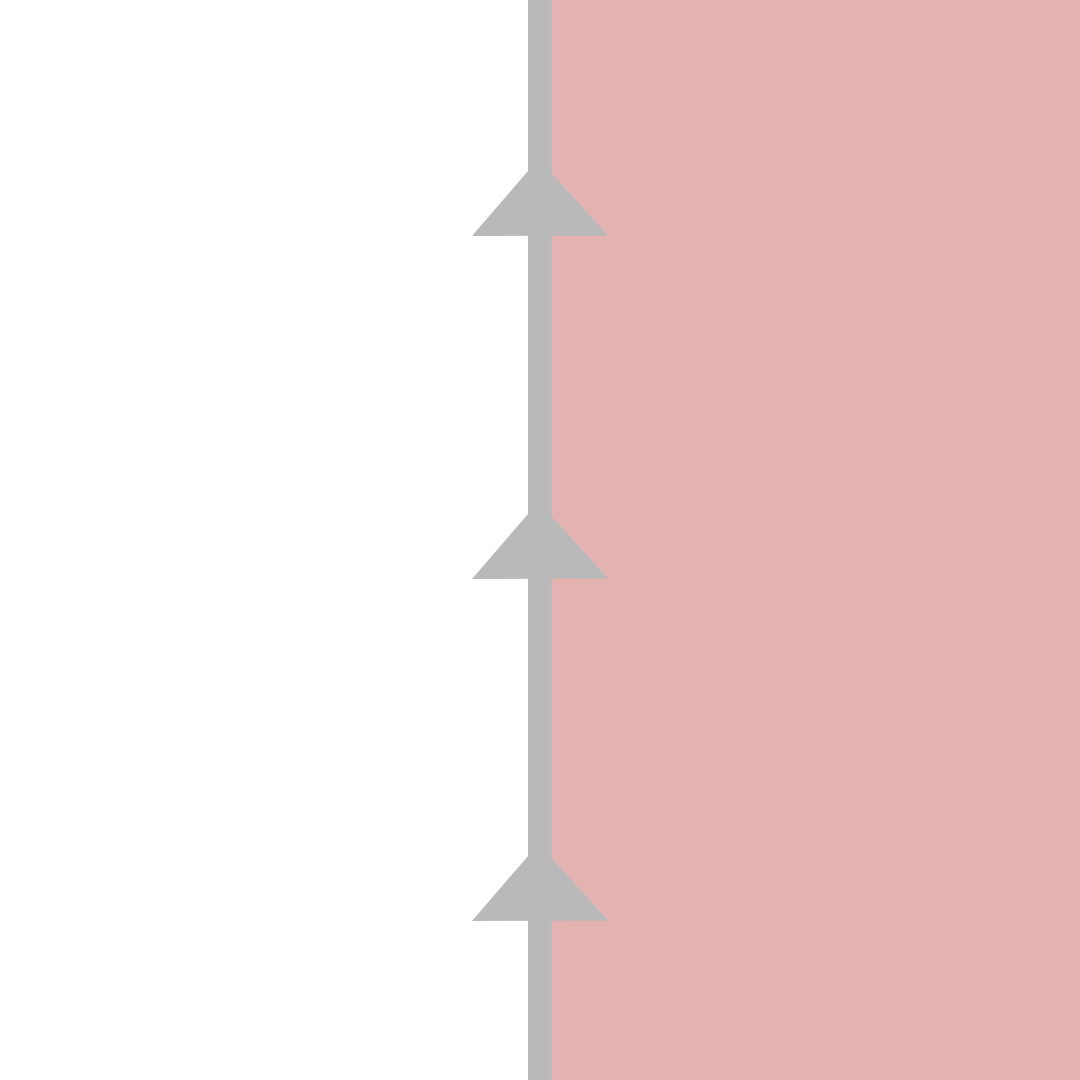
\includegraphics[width=.5\linewidth]{imgs/Mass kink Bound state.png}}
\caption{Symbolic image of a chiral zero energy bound state (Grey) localised at the interface of a region (red) topologically different to the other region (white)}
\endminipage\hspace{1cm}
\minipage[t]{0.4\textwidth}
\centering
\fcolorbox{black}{white}{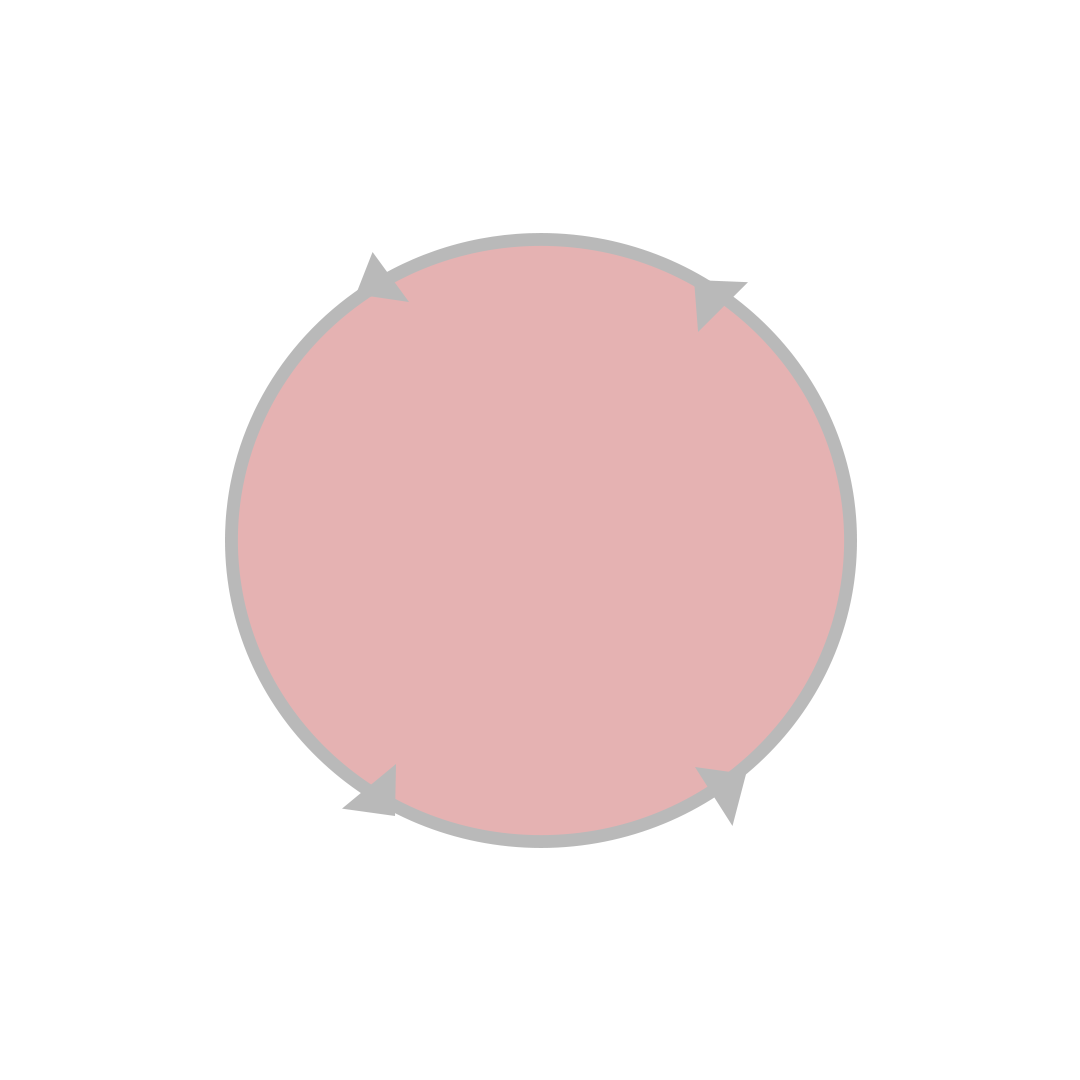
\includegraphics[width=.5\linewidth]{imgs/Majorana Bound state.png}}
\caption{Symbolic image of a chiral zero energy bound state (grey) localised around a  region (red) topologically different to the outside (white)}
\endminipage
\end{figure}
  When the interface is circular enclosing a finite topologically different region, 
  the different phase of the superconducting order parameter in $x$ and $y$ direction acts as an anti periodic boundary condition on the quasi particle wave function of states localised at the interface and no zero-energy modes can exist \cite{ivanov2001non}. The boundary conditions can be shifted by a $2\pi$ phase winding of the order parameter $\Delta$ around the centre of the region, as the phase of the order parameter of pair creation/annihilation tangentially to the edge. Physically, this phase winding can be interpreted as the Aharonov-Bohm \cite{aharonov1959significance} phase of a $\pi$-flux. Similar to a magnetic flux through a vortex pinning a type II superconductor, hence we further refer to these regions of different chemical potential with a phase winding of the order parameter around them as vortices. For such vortices the boundary conditions becomes periodic and zero energy modes are allowed. When the vortex is topologically trivial and the surrounding bulk is chiral$\pm$, a zero-energy mode is predicted. However, when the topological phase is on the inside no zero modes are predicted. When compared to the open interface of infinite regions, the enclosed region has the benefit of localising the zero-energy mode which allows for the exchange of vortices and therefor the bogoliubov quasi particles. These chiral Majorana Fermions \cite{ivanov2001non} have non abelian statistics see \secref{sec:NonAbelian}.  When two such vortices are close an exponential energy splitting results and when the radius of the vortices goes to zero the non-zero-energy modes in the superconducting gap are expected to move away from zero energy.  When only a single vortex is present the domain's boundary hosts the second mode as Majorana modes always exist in pairs. When an even number of vortices is present, the Berry phase \secref{sec:BerryPhase} suppresses the formation of a Majorana mode at the boundary. Further information in \cite{volovik1999fermion} \cite{ivanov2001non} \cite{stone2004edge}

\subsection{Non Abelian Exchange Statistics}\label{sec:ExhcangeStat}
A zero energy mode is created and destroyed by a pair of operators $d,d^{\dag}$. These can be transformed into the Majorana modes $\gamma_{a}, \gamma_{b}$, such that
$$
\frac{1}{2} \left(
\begin{array}{cc}
 1 & i \\
 1 & -i \\
\end{array}
\right) \left(
\begin{array}{c}
 \gamma _{A} \\
 \gamma _{B} \\
\end{array}
\right)=\left(
\begin{array}{c}
 d \\
 d^{\dagger } \\
\end{array}
\right)
$$
$$
\left(
\begin{array}{cc}
 1 & 1 \\
 -i & i \\
\end{array}
\right) \left(
\begin{array}{c}
 d \\
 d^{\dagger } \\
\end{array}
\right)=\left(
\begin{array}{c}
 \gamma _{A} \\
 \gamma _{B} \\
\end{array}
\right)
$$
$$
\left\lbrace
\gamma_{a/b,k}^{\dag},\gamma_{a/b,k'}
\right\rbrace
=2\delta_{k,k'}; \gamma_A = \gamma_A^{\dag},\gamma_B = \gamma_B^{\dag} $$
This implies $\gamma_A^2 = \gamma_B^2 = \mathbb{1}$. As these Majorana modes are localised,
they perform a quasi particle exchange when we move the vortices locating them around each other.
We write the unitary transformation describing the exchange corresponding to a braid $\sigma_i$  as $tau(\sigma_i)$. This transformation can also be thought of as the Time evolution operator of an ideal adiabatic exchange.
The operators $\gamma_A, \gamma_B$ transform as 
$$
\tau(\sigma_1) = \exp \left( \frac{\pi}{4} \gamma_B\gamma_A\right) = \frac{1}{\sqrt{2}} (\mathbb{1} + \gamma_B\gamma_A) 
$$
Under exchange of the vortices locating these modes, the vector $(\gamma_A,\gamma_B)^T$ transforms as \cite{chung2007stability}

$$
\tau(\sigma_1)
\left(
\begin{array}{c}
      \gamma_A \\
      \gamma_B
\end{array}
\right) = 
\left(
\begin{array}{c}
      \gamma_B \\
      -\gamma_A
\end{array}
\right)
= 
\left(
\begin{array}{cc}
   0  &  1\\
   -1  & 0
\end{array}
\right)
\left(
\begin{array}{c}
      \gamma_A \\
      \gamma_B
\end{array}
\right)
$$

This exchange matrix is similar (transposed) to the one described in \secref{sec:AnyonsCaseStudy}.
Expressed as unitary projector of the states $ \ket{0}, \ket{1} := d^{\dag}\ket{0}$.
\begin{dmath}\label{eq:2VortExchange}
 \tau(\sigma_1) = exp \left( i \frac{\pi}{4} (2d^{\dag}d - \mathbb{1})\right) = exp(i \frac{i \pi}{4} \sigma^z)
 = 
 \left(\begin{array}{cc}
      \ket{0}, \ket{1} \\
\end{array}\right)
 \left(
\begin{array}{cc}
   exp(-\frac{i \pi}{4})  &  0\\
   0  & exp(\frac{i \pi}{4})
\end{array}
\right)
\left(\begin{array}{c}
      \bra{0} \\
      \bra{1}
\end{array}\right)
\end{dmath}
Here $\sigma^z$ is the Pauli matrix in the basis $(\ket{0}, d^{\dag}\ket{0})^T$\\
In the case of four vortices, there are four Majorana modes $\gamma_{A,1} , \gamma_{B,1}, \gamma_{A,2} , \gamma_{B,2}$ with a given choice of two fermionic quasi particles $d_1 = \gamma_{A,1} + i \gamma_{B,1}, d_2 = \gamma_{A,2} + i \gamma_{B,2}$ analogous for the destruction operators. Another choice for the pairing of the modes is also ppossible, but behaves analogously. All possible exchanges are described by the Braidgroup $\mathcal{B}_4$ with its three generators $\sigma_1,\sigma_2,\sigma_2$. $\sigma_1$ describes the exchange of the modes that constitute $c_1$ while $\sigma_3$ describe the exchange of the modes that constitute $c_2$ . $\sigma_2$ is different: It exchanges Majorana modes from both $c_1$ and $c_2$. In general, the index of $\sigma_i$ depends on the choice of pairing $\gamma_A \gamma_B$ into quasi particles.
The exchange-statistics behave as unitary projector on the states $ \ket{0}, \ket{1,0} := d_1^{\dag}\ket{0},\ket{0,1} := d_2^{\dag}\ket{0},\ket{1,1} := d_2^{\dag}d_1^{\dag}\ket{0} $$
$ as can be seen from
$$\tau(\sigma_1) = exp \left( \frac{\pi}{4} \gamma_{B,1}\gamma_{A,1}\right) = \frac{1}{\sqrt{2}} (\mathbb{1} + \gamma_{B,1}\gamma_{A,1}) = exp \left( i \frac{\pi}{4} (2d_1^{\dag}d_1 - \mathbb{1})\right) 
$$
$$= 
\left(
\begin{array}{cccc}
     \ket{0} & \ket{1,0} & \ket{0,1} & \ket{1,1}
\end{array}
\right)
\left(
\begin{array}{cccc}
   e^{-\frac{i \pi}{4}}  &  0 & 0 & 0 \\
   0  & e^{\frac{i \pi}{4}}& 0 & 0 \\
    0 & 0 &e^{-\frac{i \pi}{4}}  &  0\\
    0 & 0 &0  & e^{\frac{i \pi}{4}}
\end{array}
\right)
\left(
\begin{array}{c}
     \bra{0}\\
     \bra{1,0}\\
     \bra{0,1}\\
     \bra{1,1}
\end{array}
\right)
$$
$$
\tau(\sigma_3) = exp \left( \frac{\pi}{4} \gamma_{B,2}\gamma_{A,2}\right) = \frac{1}{\sqrt{2}} (\mathbb{1} + \gamma_{B,2}\gamma_{A,2}) = exp \left( i \frac{\pi}{4} (2d_2^{\dag}d_2 - \mathbb{1})\right) 
$$
$$= 
\left(
\begin{array}{cccc}
     \ket{0} & \ket{1,0} & \ket{0,1} & \ket{1,1}
\end{array}
\right)
\left(
\begin{array}{cccc}
   e^{-\frac{i \pi}{4}}  &  0 & 0 & 0 \\
   0  & e^{-\frac{i \pi}{4}}& 0 & 0 \\
    0 & 0 &e^{\frac{i \pi}{4}}  &  0\\
    0 & 0 &0  & e^{\frac{i \pi}{4}}
\end{array}
\right)
\left(
\begin{array}{c}
     \bra{0}\\
     \bra{1,0}\\
     \bra{0,1}\\
     \bra{1,1}
\end{array}
\right)
$$
$$
\tau(\sigma_2) = exp \left( \frac{\pi}{4} \gamma_{B,1}\gamma_{A,2}\right) = \frac{1}{\sqrt{2}} (\mathbb{1} + \gamma_{B,1}\gamma_{A,2}) = \frac{1}{\sqrt{2}} \left( \mathbb{1} + i (d^{\dag}_2 + d_2)(d^{\dag}_1 - d_1)  \right)$$
\begin{dmath}\label{math:UnusualEchchange}=
\left(
\begin{array}{cccc}
     \ket{0} & \ket{1,0} & \ket{0,1} & \ket{1,1}
\end{array}
\right)
\frac{1}{\sqrt{2}}
\left(
\begin{array}{cccc}
   1  &  0 & 0 & - i \\
   0  & 1 & - i & 0 \\
    0 & -i & 1  &  0\\
    -i & 0 & 0  & 1
\end{array}
\right)
\left(
\begin{array}{c}
     \bra{0}\\
     \bra{1,0}\\
     \bra{0,1}\\
     \bra{1,1}
\end{array}
\right)
\end{dmath}
\end{document}